\documentclass{elsarticle}\usepackage[]{graphicx}\usepackage[]{color}
%% maxwidth is the original width if it is less than linewidth
%% otherwise use linewidth (to make sure the graphics do not exceed the margin)
\makeatletter
\def\maxwidth{ %
  \ifdim\Gin@nat@width>\linewidth
    \linewidth
  \else
    \Gin@nat@width
  \fi
}
\makeatother

\definecolor{fgcolor}{rgb}{0.345, 0.345, 0.345}
\newcommand{\hlnum}[1]{\textcolor[rgb]{0.686,0.059,0.569}{#1}}%
\newcommand{\hlstr}[1]{\textcolor[rgb]{0.192,0.494,0.8}{#1}}%
\newcommand{\hlcom}[1]{\textcolor[rgb]{0.678,0.584,0.686}{\textit{#1}}}%
\newcommand{\hlopt}[1]{\textcolor[rgb]{0,0,0}{#1}}%
\newcommand{\hlstd}[1]{\textcolor[rgb]{0.345,0.345,0.345}{#1}}%
\newcommand{\hlkwa}[1]{\textcolor[rgb]{0.161,0.373,0.58}{\textbf{#1}}}%
\newcommand{\hlkwb}[1]{\textcolor[rgb]{0.69,0.353,0.396}{#1}}%
\newcommand{\hlkwc}[1]{\textcolor[rgb]{0.333,0.667,0.333}{#1}}%
\newcommand{\hlkwd}[1]{\textcolor[rgb]{0.737,0.353,0.396}{\textbf{#1}}}%

\usepackage{framed}
\makeatletter
\newenvironment{kframe}{%
 \def\at@end@of@kframe{}%
 \ifinner\ifhmode%
  \def\at@end@of@kframe{\end{minipage}}%
  \begin{minipage}{\columnwidth}%
 \fi\fi%
 \def\FrameCommand##1{\hskip\@totalleftmargin \hskip-\fboxsep
 \colorbox{shadecolor}{##1}\hskip-\fboxsep
     % There is no \\@totalrightmargin, so:
     \hskip-\linewidth \hskip-\@totalleftmargin \hskip\columnwidth}%
 \MakeFramed {\advance\hsize-\width
   \@totalleftmargin\z@ \linewidth\hsize
   \@setminipage}}%
 {\par\unskip\endMakeFramed%
 \at@end@of@kframe}
\makeatother

\definecolor{shadecolor}{rgb}{.97, .97, .97}
\definecolor{messagecolor}{rgb}{0, 0, 0}
\definecolor{warningcolor}{rgb}{1, 0, 1}
\definecolor{errorcolor}{rgb}{1, 0, 0}
\newenvironment{knitrout}{}{} % an empty environment to be redefined in TeX

\usepackage{alltt}
\usepackage[top=1in, left=1in, right=1in, bottom=1in]{geometry}

\usepackage{float, amsmath}
\usepackage{tikz}
\usetikzlibrary{shapes,arrows}
\usetikzlibrary{positioning}
\usepackage{float, amsmath}
\usepackage{url}
\usepackage{enumerate}
\usepackage{natbib}


%\usepackage[
%  natbib = true,
%    backend=bibtex,
%    isbn=false,
%    url=false,
%    doi=false,
%    eprint=false,
%    style=numeric,
%    sorting=nyt,
%    sortcites = true
%]{biblatex}
%\bibliography{CT_Pipeline_l}
%\bibliography{CT_Skull_Stripping}


\usepackage{subfig}










%\usepackage[all]{hypcap}
\IfFileExists{upquote.sty}{\usepackage{upquote}}{}
\begin{document}
\renewcommand{\thesubfigure}{\Alph{subfigure}}

\begin{frontmatter}

\date{}

\title{Validated Automatic Brain Extraction of Head CT Images using FSL-Brain Extraction Tool (BET)}
%\title{Validated Automatic Brain Extraction of Head CT Images using Established, Open-Source, Neuroimaging Software}

\author[jhsph]{John~Muschelli\corref{cor1}}
\ead{jmusche1@jhu.edu}

\author[jhmi]{Natalie~Ullman}
\ead{nullman1@jhmi.edu}

\author[jhsph]{Ciprian~M.~Crainiceanu}
\ead{ccrainic@jhsph.edu}

\cortext[cor1]{Principal Corresponding Author}
\address[jhsph]{Department of Biostatistics, Bloomberg School of Public Health, Johns Hopkins University, Baltimore, MD, USA}
\address[jhmi]{Department of Neurology, Division of Brain Injury Outcomes,  Johns Hopkins Medical Institutions, Baltimore, MD, USA}

\begin{abstract}
\section{Background}
Computed Tomography (CT) brain imaging is commonly used in diagnostic settings.  Although CT scans are primarily used in a clinical setting, they can be used to answer research hypotheses.  Methods for brain extraction in head CT images has been informally proposed, but never formally validated.


\section{Aim}

To systematically analyze the performance of FSL's brain extraction tool (BET) on head CT images of patients with intracranial hemorrhage by varying its parameters and options after performing CT-specific preprocessing, and quantitatively comparing its results to a manual gold standard.

\section{Methods}

Nineteen images from 16 patients with intracranial hemorrhage were selected from 13 different MISTIE stroke trial centers. Before running BET, the image was: (1) not smoothed or smoothed using a $1$mm Gaussian smoother, (2) thresholded to $0-100$ Hounsfield units (HU), (3) BET was applied using 1 of 3 fractional intensity (FI) thresholds: $0.01$, $0.1$, $0.35$, (4) holes in the mask were filled.
For comparison, intracranial masks were manually created for all image volumes from expert CT readers.  The resulting brain tissue masks were quantitatively compared to the manual segmentations using sensitivity, specificity, accuracy, and the Dice Similarity Index (DSI).  Different results were compared using Wilcoxon signed-rank tests.

\section{Results}

Without smoothing the images, BET performed poorly regardless of FI.  After smoothing, performance was high for all metrics for all scans.  All reported measures are on smoothed data.  Using an FI of $0.01$ or $0.1$ performed better than $0.35$; we will focus and compare these FI.  Using an FI of $0.01$ had a higher median sensitivity ($0.9921$) than an FI of $0.1$ ($0.9905$, $p< 0.001$), lower specificity ($0.9979$ vs. $0.998$; $p< 0.001$), , and no difference in accuracy ($0.9971$ vs. $0.9971$; $p= 0.134$) or DSI ($0.9894$ vs. $0.9896$; $p= 0.066$).  Overall, regardless of p-values, these measures are all high in practice and largely adequate for good brain extraction.

\section{Conclusion}

BET performs well at brain extraction on thresholded, $1$mm smoothed CT images with an FI of $0.01$.  Smoothing before applying BET is an important step not previously discussed.  Analysis code is provided.

\end{abstract}
\maketitle
\begin{keyword}
CT \sep skull stripping \sep brain extraction \sep validation
\end{keyword}

\end{frontmatter}



\section{Introduction}

X-ray computed tomography (CT) scanning is widely available and is a commonly used diagnostic tool in clinical settings \citep{sahni_management_2007}. Though much analysis of CT images are done by qualitative visual inspection, detailed quantification of information is of interest.  CT scans do not discriminate in the tissues or structures captured; scans have non-brain structures such as the skull, eyes, facial and nasal features, extracranial skin, and more importantly non-human elements captured by the scanner, such as pillows or medical devices.  These objects present a problem for extracting metrics on brain tissue.  We propose a validated automated solution to brain extraction in head CT scans using established neuroimaging software.

In magnetic resonance imaging (MRI), brain extraction has been extensively studied and investigated (see \citet{wang2014knowledge} for an extensive list).  As such, many pieces of software and algorithms exist to achieve this goal with respect to MRI scans.  We have adapted one algorithm, the Brain Extraction Tool (BET) \citep{smith_fast_2002}, a function of the FSL \citep{jenkinson_fsl_2012} neuroimaging software (v5.0.4), to automatically extract the brain from a CT scan.  Variations of this pipeline have been presented before in \citet{able}, and has been replicated in slightly more detail in \citet{rorden_age-specific_2012}.  Neither presented a formal validation against a set of manually segmented brain images, which is the goal of our study. 


\section{Methods}
\subsection{ Participants and CT data}
We used CT images patients enrolled in the MISTIE (Minimally Invasive Surgery plus recombinant-tissue plasminogen activator for Intracerebral Evacuation) and ICES (Intraoperative CT-Guided Endoscopic Surgery) trials.  These patients had an intracranial hemorrhage at time of scanning; for inclusion criteria, see \citet{mould_minimally_2013}. CT data were collected as part of the Johns Hopkins Medicine IRB-approved MISTIE research studies with written consent from participants.  


\subsection{Imaging Data}
The study protocol was executed with minor, but important, differences across the 13 sites.  
%%% nEEED TO ADD
%Scans were acquired using manu[1] ($N=man.tab[1]$), manu[2] ($N=man.tab[2]$), manu[3] ($N=man.tab[3]$), and manu[4] ($N=man.tab[4]$) scanners. Gantry tilt was observed in n.gant scans.  
Slice thickness of the image varied within the scan for 2 scans, referred to as variable slice thickness. For example, a scan may have 10 millimeter (mm) slices at the top and bottom of the brain but with 5mm slices in the middle of the brain.  Therefore, the scans analyzed had different voxel (volume element) dimensions and image resolution prior to registration to the template.  These conditions represent how scans are presented for evaluation in many diagnostic cases.

%Different reconstructions of CT images are not available via the data-acquiring center, and 

\subsection{Manual and Automated Brain Extraction}
We analyzed 19 scans, corresponding to 16 unique patients.  Brain tissue was manually segmented as a binary mark from DICOM (Digital Imaging and Communications in Medicine) images in the OsiriX imaging software (OsiriX v.4.1, Pixmeo; Geneva, Switzerland) by one expert reader (NU). 
CT brain images and the binary mask were exported from OsiriX to DICOM format.  Images with gantry tilt were corrected using a customized MATLAB (The Mathworks, Natick, Massachusetts, USA) user-written script (\url{http://bit.ly/1ltIM8c}). 
Images were converted to the Neuroimaging Informatics Technology Initiative (NIfTI) data format using \verb|dcm2nii| (2009 version, provided with MRIcro \citep{rorden_stereotaxic_2000}).  Images were constrained to values $-1024$ and $3071$ HU to remove potential image rescaling errors and artifacts.  No interpolation was done for images with a variable slice thickness. Thickness was determined from the first slice converted and was assumed homogeneous throughout the image.  The image processing pipeline can be seen in Figure~\ref{fig:framework}.



\tikzstyle{bblock} = [rectangle, draw, text width=8em, text centered, minimum height=3em, rounded corners]
\tikzstyle{line} = [draw, text centered , -latex']
\tikzstyle{line node} = [draw, fill=white, font=\tiny ]
\tikzstyle{block} = [rectangle, draw, text width=5em, text centered, minimum height=4em, rounded corners]    

\begin{figure}
\centering
\begin{tikzpicture}[node distance = 2cm, every node/.style={rectangle,fill=white}]
% Place nodes
\node [bblock] (raw) {DICOM images};
\node [bblock, below of=raw] (dcmnii) {NIfTI image };
\node [bblock, below of=dcmnii, left of=dcmnii] (nosmooth) {No Smooth};
\node [bblock, below of=dcmnii, right of=dcmnii] (smooth) {Smooth ($1$mm)};

\node [bblock, below of=nosmooth, right of=nosmooth] (BET) {BET};

\node [block, below of=BET, node distance = 3cm] (SS_1) {FI=0.1};
\node [block, left = 1.75em of SS_1] (SS_01) {FI=0.01};
\node [block, right = 1.75em of SS_1] (SS_35) {FI=0.35};

\node [block, below of=SS_1, node distance = 2cm] (Fillin) {Use FSL to fill mask holes};

\node [block, below of=Fillin, node distance = 2cm] (Measures) {Performance Measures};


% Draw edges
\path [line] (raw) -- node {dcm2nii} (dcmnii);
\path [line] (dcmnii) -- (nosmooth);
\path [line] (dcmnii) -- (smooth);
\path [line] (smooth) -- (BET);
\path [line] (nosmooth) -- (BET);
\path [line] (BET) -- (SS_01);
\path [line] (BET) -- (SS_35);
\path [line] (BET) -- node {Different FI Value} (SS_1);
\path [line] (SS_1) -- (Fillin);
\path [line] (SS_01) -- (Fillin);
\path [line] (SS_35) -- (Fillin);
\path [line] (Fillin) -- (Measures);
\end{tikzpicture}
\caption{Overall workflow of processing of data.  After the raw data has been processed and areas have been extracted, surfaces can be rendered.  We are concerned with those steps in orange: creating surfaces, and export to the web.  The last branch shows 2 options for export: publishing the figure to the web or enclosing it in a folder with all tools to render it.  The second option would allow users to include these zipped directories as supplementary figures until more widely used.   }
\label{fig:framework}
\end{figure}

Images were thresholded to a brain tissue range ($0$-$100$ HU).
We either applied BET to the this image or smoothed this image with a Gaussian kernel ($\sigma=1$mm, using FSL), re-thresholded to $0$-$100$ HU and then applied BET.  When BET was applied, we varied fractional intensity (FI) parameter to determine its influence on performance: we used values of $0.35$ (as recommended in \citet{rorden_age-specific_2012}), $0.1$, $0.01$.  

We also present one example case which demonstrates that brain extraction performance was acceptable only after smoothing before BET was applied.  


\subsection{Measuring and Testing Brain Extraction Performance}
Five common measurements of performance were calculated for each image: sensitivity, specificity, accuracy, and the Dice Similarity Index (DSI).  See Inline Supplementary Methods 1 for the calculation of each measure.

[Insert Supplementary Methods 1 here]

Performance was compared across FI using Wilcoxon signed-rank tests.



%and the Jaccard index is defined as:
%$$
%\frac{ \sum_{i=1}^{V} \left( I_{ia} \times I_{im}\right) }{\sum_{i=1}^{V} I_{ia}  + \sum_{i=1}^{V} I_{im} - \sum_{i=1}^{V} \left(I_{ia} \times I_{im} \right)}
%$$

\section{Results}
Figure~\ref{fig:metrics}\protect\subref*{unsmoothed} illustrates the performance of each variation of the BET pipeline in Figure~\ref{fig:framework}.  The smoothed pipelines perform better than the unsmoothed pipelines and BET performs poorly on some scans without smoothing.  

Figure~\ref{fig:metrics}\protect\subref*{smoothed} displays the performance for brain extraction in the smoothed pipelines (note the change in the y-axis).  After smoothing, performance was high for all metrics for all scans.  All reported measures are on smoothed data.  
Using an FI of $0.01$ or $0.1$ performed better than $0.35$; we will focus and compare these FI.  Using an FI of $0.01$ had a higher median sensitivity ($0.9921$) than an FI of $0.1$ ($0.9905$, $p< 0.001$), lower specificity ($0.9979$ vs. $0.998$; $p< 0.001$), , and no difference in accuracy ($0.9971$ vs. $0.9971$; $p= 0.134$) or DSI ($0.9894$ vs. $0.9896$; $p= 0.066$).  Overall, regardless of p-values, these measures are all high in practice and largely adequate for brain extraction.

% Overall, using an FI of $0.35$ performs worse overall than $0.01$ or $0.1$ for all measures other than specificity.  
% 
% Without smoothing the images, BET performed poorly regardless of FI.  
% 












\begin{figure}
  \subfloat{
  \label{smoothed}
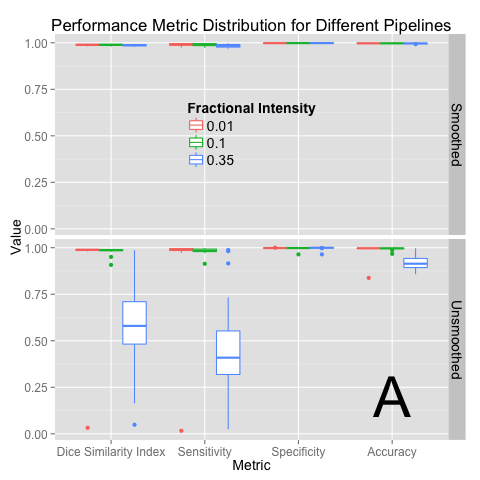
\includegraphics[width=.48\textwidth]{figure/CT_Skull_Stripping_Figure2.png}
}
\hfill
  \subfloat{
  \label{unsmoothed}
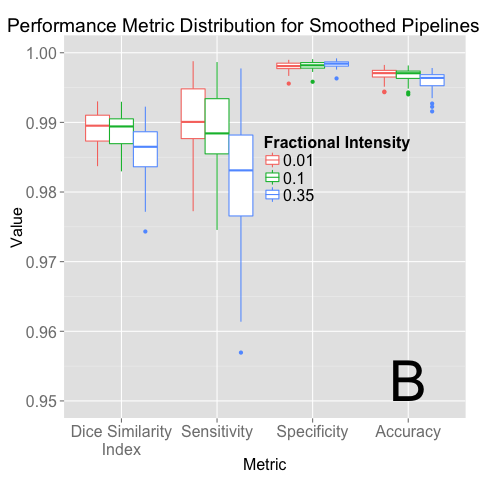
\includegraphics[width=.48\textwidth]{figure/CT_Skull_Stripping_Figure2b.png}
}
\caption{{\bf Performance Metric Distribution for Different Pipelines.} Panel~\protect\subref*{smoothed} displays the boxplots for performance measures when running the pipeline with a different fractional intensity (FI), using smoothed data (top) or unsmoothed data (bottom).  Panel~\protect\subref*{unsmoothed} presents the smooothed data only, rescaled to show discrimination between the differernt FI.Overall, FI of $0.01$ and $0.1$ perform better than $0.35$ in all categories other than specificity.  Using smoothed data improves performance in all performance metrics, markedly when an FI of $0.35$ is used.  Panel~\protect\subref*{unsmoothed} demonstrates that using an FI of $0.01$ on smoothed data is the best pipeline.  }
\label{fig:metrics}
\end{figure}


Although Figure~\ref{fig:metrics} displays that using FI of $0.01$ or $0.1$ provides adequate results of brain extraction for most cases, they perform relatively well regardless of smoothing the data.  Figure~\ref{fig:ss_example} displays an example where using unsmoothed data performs poorly for these FI, demonstrating why smoothing is essential for a general brain extraction procedure for CT.

\begin{figure}[H]
\centering
  \subfloat{
  \label{ss:01_smooth}
	\includegraphics[width=.31\textwidth]{figure/{101-307_20061110_1638_CT_5_RM_Head_SS_0.01_Mask}.png} 
}
\hfill
  \subfloat{
  \label{ss:1_smooth}
	\includegraphics[width=.31\textwidth]{figure/{101-307_20061110_1638_CT_5_RM_Head_SS_0.1_Mask}.png} 
}
\hfill
  \subfloat{
  \label{ss:35_smooth}
	\includegraphics[width=.31\textwidth]{figure/{101-307_20061110_1638_CT_5_RM_Head_SS_0.35_Mask}.png} 
}
\newline
\hfill 
  \subfloat{
  \label{ss:01_nosmooth}
	\includegraphics[width=.31\textwidth]{figure/{101-307_20061110_1638_CT_5_RM_Head_SS_0.01_nopresmooth_Mask}.png} 
}
\hfill
  \subfloat{
  \label{ss:1_nosmooth}
	\includegraphics[width=.31\textwidth]{figure/{101-307_20061110_1638_CT_5_RM_Head_SS_0.1_nopresmooth_Mask}.png} 
}
\hfill
  \subfloat{
  \label{ss:35_nosmooth}
	\includegraphics[width=.31\textwidth]{figure/{101-307_20061110_1638_CT_5_RM_Head_SS_0.35_nopresmooth_Mask}.png} 
}
\caption{{\bf Example Demonstrating How Smoothing Prior to BET is Essential} For one subject, the CT image is displayed with the brain extracted mask in red after running all pipelines.  Panels~\protect\subref*{ss:01_smooth}, \protect\subref*{ss:1_smooth}, and \protect\subref*{ss:35_smooth} represent applying BET using FI of $0.01$, $0.01$, and $0.35$, respectivley, to smoothed data. Panels~\protect\subref*{ss:01_nosmooth}, \protect\subref*{ss:1_nosmooth}, and \protect\subref*{ss:35_nosmooth} correspond to applying BET using FI $0.01$, $0.01$, and $0.35$ on unsmoothed data.  Using smoothed data is required for adequate brain extraction.
}
\label{fig:ss_example}
\end{figure}

\section{Conclusions}
We present an automated brain extraction pipeline for CT images that was validated using gold-standard manual segmentations of brain tissues.  Overall, we found that smoothing the data with a conservative smoother ($1$mm Gaussian kernel) and using an FI of $0.01$ provides good brain extraction for the sample studied.  We believe this pipeline is generalized for most brain CT scans.  These software (FSL and R) are freely available to download under public licenses are open source.  Thus, this pipeline should be widely available. 

With the resulting automated brain masks output from this pipeline, researchers can now do within-tissue operations, such as intensity normalization, brain volume estimation, tissue/tumor/hemorrhage segmentation, etc. 

The \texttt{R} function to perform brain extraction is located at \url{https://github.com/muschellij2/CT_BET/blob/master/Skull_Strip_Paper/CT_Skull_Strip_Example.R}. 


\section*{Inline Supplementary Methods 1}
Let $I_{ia}, I_{im}$ be the indicators that voxel $i$ for the automatic and manual masks, respectively, such that $I_{i} = 1$ if voxel $i$ is labeled in the brain mask and $0$ otherwise.  

A true positive (TP) is defined when: $I_{ia} = 1$ and $I_{im} = 1$, a false positive (FP): $I_{ia} = 1$ and $I_{im} = 0$, a false negative (FN): $I_{ia} = 0$ and $I_{im} = 1$, and a true negative (TN): $I_{ia} = 0$ and $I_{im} = 0$.
Sensitivity is defined as
$$
\frac{\# \text{TP} }{\# \text{TP} + \text{FN}} = \frac{ \sum_{i=1}^{V} \left( I_{ia} \times I_{im}\right) }{ \sum_{i=1}^{V} I_{im}}
$$
and specificity is defined as
$$
\frac{\# \text{TN} }{\# \text{TN} + \text{FP}} = \frac{ \sum_{i=1}^{V} \left( (1-I_{ia}) \times (1- I_{im} ) \right) }{ \sum_{i=1}^{V} (1 - I_{im} )}
$$
and overall accuracy is:
$$
\frac{\# \text{TN} + \text{TP} }{\# \text{TN} + \text{FN} + \text{TP} + \text{FP}} = \frac{ \sum_{i=1}^{V} (I_{ia} \times I_{im}) + \left( (1-I_{ia}) \times (1- I_{im} ) \right) }{\sum_{i=1}^{V} I_{ia}  + \sum_{i=1}^{V} I_{im}}
$$


The Dice Similarity Index is defined as:
$$
\frac{2 \times \#\text{TP} }{ \# \text{TN} + \text{FN} + \text{TP} + \text{FP}} = \frac{ 2 \times \sum_{i=1}^{V} \left( I_{ia} \times I_{im}\right) }{\sum_{i=1}^{V} I_{ia}  + \sum_{i=1}^{V} I_{im}}
$$


\newpage
\section*{References}
\bibliographystyle{elsarticle-num-names}
\bibliography{CT_Skull_Stripping}
%\printbibliography



\end{document}
